% Copyright Aidan Randle-Conde 2007-2014
% http://www.aidansean.com/phd_notes
% Anyone is free to download, redistribute, edit and use these notes and the source tex files with the following restrictions:
% This 
%  This message is included in the tex source files.
%  Aidan Randle-Conde is credited as the author.
%  Images are correctly credited to their respective authors, as outlined in the references.
%  No part of these notes may be used for commercial purposes.

\chapter{Review of non relativistic quantum mechanics}
\chaptermark{Non-relativistic quantum mechanics}

\section{Schroedinger picture and probability current}

For a free particle of mass $m$ the classical energy-momentum relation is:

\[
  E = \frac{p^2}{2m}
\]

In quantum mechanics, $p$ and $E$ become differential operators:

\begin{eqnarray*}
  E & \to & 1\frac{\partial}{\partial t} \\
  p & \to & -i \nabla \\
  ( \hbar & = & 1 )
\end{eqnarray*}

These operate on the wavefunction:

\begin{eqnarray}
  \frac{(-i)^2}{2m}\nabla^2 \psi & = & i \frac{\partial}{\partial t}\psi \nonumber \\
  \frac{-1}{2m}\nabla^2\psi & = & i\frac{\partial \psi}{\partial t} \label{eq:schroedinger1} \\
  \psi^{\star} \times (\ref{eq:schroedinger1}) :\quad \frac{-1}{2m} \psi^{\star}\nabla^2\psi & = & i\psi^{\star}\frac{\partial \psi}{\partial t} \label{eq:schroedinger2} \\
  \textrm{Complex conjugate of (\ref{eq:schroedinger1}): } \frac{-1}{2m}\nabla^2\psi^{\star} & = & -i\frac{\partial \psi^{\star}}{\partial t} \label{eq:schroedinger3} \\
  \psi \times (\ref{eq:schroedinger3}) :\quad \frac{-1}{2m}\psi\nabla^2\psi^{\star} & = & -i\psi\frac{\partial \psi^{\star}}{\partial t} \label{eq:schroedinger4} \\
  (\ref{eq:schroedinger2}) - (\ref{eq:schroedinger4}) & = & i\left( \psi^{\star}\frac{\partial \psi}{\partial t} + \psi\frac{\partial \psi^{\star}}{\partial t} \right) \nonumber \\
  & = & \frac{-1}{2m}\left(\psi^{\star}\nabla^2\psi - \psi\nabla^2\psi^{\star}\right) \nonumber \\
  \textrm{So } i\left(\psi^{\star}\frac{\partial \psi}{\partial t} + \psi\frac{\partial \psi^{\star}}{\partial t}\right) & = & \frac{-1}{2m}\left(\psi^{\star}\nabla^2\psi - \psi\nabla^2\psi^{\star}\right) \nonumber \\
  \textrm{or } \frac{\partial}{\partial t}\left(\psi^{\star}\psi\right) + \frac{i}{2m}\left(\psi\nabla^2\psi^{\star} - \psi^{\star}\nabla^2\psi \right) & = & 0 \nonumber \\
  \frac{\partial}{\partial t}\left(\psi^{\star}\psi\right) + \frac{i}{2m}\ul{\nabla}\cdot\left(\psi\ul{\nabla}\psi^{\star} - \psi^{\star}\ul{\nabla}\psi\right) & = & 0 \nonumber \\
  \frac{\partial}{\partial t}\int_V\left(\psi^{\star}\psi\right) \mathrm{d}V + \frac{i}{2m}\int_V \ul{\nabla}\cdot\left(\psi\ul{\nabla}\psi^{\star}-\psi\ul{\nabla}\psi\right) \mathrm{d}V & = & 0 \label{eq:schroedinger5}
\end{eqnarray}

(\ref{eq:schroedinger5}) resembles a conservation equation of the form:

\[
  \frac{\partial \rho}{\partial t} + \ul{\nabla}\cdot\ul{J} = 0
\]

where:

\begin{eqnarray*}
  \ul{J} & = & \frac{i}{2m}\left(\psi\ul{\psi}^{\star} - \psi^{\star}\ul{\nabla}\psi\right) \\
  \rho & = & |\psi|^2
\end{eqnarray*}

The divergence theorem then gives:

\[
  \frac{i}{2m}\int_S\left(\psi\ul{\nabla}\psi^{\star} - \psi^{\star}\ul{\nabla}\psi\right)\cdot\ul{\hat{n}}\mathrm{d}S = \frac{i}{2m}\int_V\left(\psi\ul{\nabla}\psi^{\star} - \psi^{\star}\ul{\nabla}\psi\right)\mathrm{d}V
\]

As an example, consider $\rho$ and $\ul{J}$ for a plane quantum wave:

\begin{eqnarray*}
  \psi & = & N\e^{i\left(px - Et\right)} \\
  \rho & = & |\psi|^2 \\
       & = & \psi^{\star}\psi \\
       & = & N\e^{i\left(px - Et\right)}N^{\star}\e^{-i\left(px - Et\right)} \\
       & = & NN^{\star} \\
       & = & |N|^2 \\
  \textrm{So: } \rho & = & |N|^2 \\
  \ul{J} & = & \frac{i}{2m}\left(\psi\ul{\nabla}\psi^{\star} - \psi\ul{\nabla}\psi\right) \\
       & = & \frac{i}{2m}\lbrace N \e^{i\left(px - Et\right)}\ul{\nabla}N^{\star}\e^{-i\left(px - Et\right)}\ul{\nabla}N\e^{i\left(px - Et\right)}\rbrace \\
       & = & \frac{i}{2m}\lbrace NN^{\star}\e^{i\left(px - Et\right)}\e^{iEt}\left(-ip\right)\e^{-ipx}
             - N^{\star}\e^{-i\left(px - Et\right)}N\e^{-iEt}\left(ip\right)\e^{ipx}\rbrace \\
       & = & \frac{i}{2m}\lbrace NN^{\star}\left(-ip\right) - N^{\star}N\left(ip\right)\rbrace \\
       & = & \frac{|N|^2}{2m}p\times 2 \\
       & = & \frac{p}{m}|N|^2
\end{eqnarray*}

In the Schroedinger picture the operators are time independent whereas the wavefunctions are time dependent.  In classical mechanics the ``operators'' (momentum and energy) are time dependent.  The Heisenberg picture gives a formulation which gives time dependent operators.

\section{The Heisenberg picture}

Starting from the Schroedinger equation:

\[
  i\frac{\partial}{\partial t}\psi(\ul{r},t) = H\psi(\ul{r},t)
\]

Also recall that the expectation of an observable, $A$, represented by the operator $\hat{A}$ is given by:

\[
  \langle \hat{A} \rangle = \int \psi^{\star}(\ul{r},t)A\psi(\ul{r},t)\mathrm{d}^3r
\]

Solving the Schroedinger equation:

\begin{eqnarray*}
  i\frac{\partial \psi(\ul{r},t)}{\partial t} & = & H\psi(\ul{r},t) \\
  i\frac{\partial \psi(\ul{r},t)}{\psi(\ul{r},t)} & = & H \partial t \\
  i\int_0^t \frac{\partial \psi(\ul{r},t)}{\psi(\ul{r},t)} & = & \int_0^t H \partial t' \\
  \Rightarrow \ln\lbrack\psi(\ul{r},t)\rbrack - \ln\lbrack\psi(\ul{r},0)\rbrack & = & -iHt \\
  \textrm{So } \frac{\psi(\ul{r},t)}{\psi(\ul{r},0)} & = & \e^{-iHt} \\
  \Rightarrow \psi(\ul{r},t) & = & \psi(\ul{r},0)\e^{-iHt}
\end{eqnarray*}

Condsider the expectation of $A$:

\begin{eqnarray*}
  \langle \hat{A} \rangle & = & \int\psi^{\star}(\ul{r},0)\e^{iHt}\hat{A}\psi(\ul{r},t)\e^{-iHt}\mathrm{d}^3r \\
  \textrm{Define }A_H & = & \e^{iHt}\hat{A}\e^{-iHt} \\
  \frac{\mathrm{d}A_H}{\mathrm{d}t} & = & iH\e^{iHt}\bar{A}\e^{-iHt} + \e^{iHt}\hat{A}(iH)\e^{-iHt} \\
  & = & i(H\hat{A} - \bar{A}H) \\
  & = & i\lbrack H , \hat{A} \rbrack
\end{eqnarray*}

In the interaction picture the time dependent perturbations are given by:

\[
  H = H_0 + H'
\]

where $H_0$ is unperturbed and $H'$ is an interaction perturbation.

\[
  \textrm{Define } H^0_I = \e^{iH_0t}H'\e^{-H_0t}
\]

This gives:

\[
  \frac{\mathrm{d}H'_I}{\mathrm{d}t} = i\lbrack H_0 , H' \rbrack
\]

\section{The harmonic oscillator}

This is a mechanical system which can be used to introduce the concept of creation annihilation operators.

\[
  H = \frac{p^2}{2m} + \frac{1}{2}m\omega^2q^2
\]

The potential energy arises because of a force proportonal to $q$:

\begin{eqnarray*}
  \textrm{Recall } F & = & -kq \\
  & = & m \frac{\mathrm{d}^2q}{\mathrm{d}t^2} \\
  \omega & = & \sqrt{\frac{k}{m}} \\
  V & = & -\int F \mathrm{d}q \\
  & = & \int kq \mathrm{d}q \\
  & = & \frac{kq^2}{2} \\
  k & = & m\omega^2 \\
  \textrm{So } V & = & \frac{m\omega^2q^2}{2}
\end{eqnarray*}

Consider the creation and annihilation operators:

\begin{eqnarray*}
  \textrm{Let } \hat{a} & = & \frac{1}{\sqrt{2}}\left(\sqrt{m\omega}\hat{q} + \frac{i}{\sqrt{m\omega}}\hat{p} \right) \\
  \hat{a}^{\dagger}     & = & \frac{1}{\sqrt{2}}\left(\sqrt{m\omega}\hat{q} - \frac{i}{\sqrt{m\omega}}\hat{p} \right)
\end{eqnarray*}

Consider the commutator given by $\lbrack \hat{q} , \hat{p} \rbrack = i$:

\begin{eqnarray*}
  \lbrack \hat{a} , \hat{a}^{\dagger} \rbrack
  & = & \frac{1}{\sqrt{2}\sqrt{2}}
        \left( m\omega \lbrack \hat{q},\hat{q} \rbrack
        + \frac{i}{\sqrt{m\omega}}\lbrack\hat{p},\hat{q}\rbrack\sqrt{m\omega} \right. \\
  &   & \left. - i\sqrt{m\omega}\lbrack\hat{q},\hat{p}\rbrack\frac{1}{\sqrt{m\omega}}
        + \frac{1}{m\omega}\lbrack\hat{p},\hat{p}\rbrack\right) \\
  & = & \frac{1}{2}\left(i(-i) - i (i) \right) \\
  & = & 1 \\
  \textrm{So } \lbrack \hat{a},\hat{a}^{\dagger}\rbrack & = & 1
\end{eqnarray*}

The Hamiltonian can be written as:

\begin{equation}
  H = \frac{\left(\hat{a}^{\dagger}\hat{a} + \bar{a}\bar{a}^{\dagger}\right)}{2}\omega \label{eq:hamiltonianSHO}
\end{equation}

To demonstrate (\ref{eq:hamiltonianSHO}):

\begin{eqnarray*}
  \hat{a}^{\dagger}\hat{a} & = & \frac{1}{\sqrt{2}}\left(\sqrt{m\omega}\hat{q} - \frac{i}{\sqrt{m\omega}}\hat{p}\right)\frac{1}{\sqrt{2}}\left(\sqrt{m\omega}\hat{q} + \frac{i}{\sqrt{m\omega}}\hat{p}\right) \\
  & = & \frac{1}{2}\left(m\omega\hat{q}^2 + \frac{\hat{p}^2}{m\omega} + 2i\left(\hat{q}\hat{p} - \hat{q}\hat{q}\right)\right) \\
  \hat{a}\hat{a}^{\dagger} & = & \frac{1}{2}\left(m\omega \hat{q}^2 + \frac{\hat{p}^2}{m\omega} + i\left(\hat{p}\hat{q} - \hat{q}\hat{p}\right)\right) \\
  \textrm{So } \hat{a}^{\dagger}\hat{a} + \hat{a}\hat{a}^{\dagger} & = & m\omega \hat{q}^2 + \frac{\hat{p}^2}{m\omega}
\end{eqnarray*}

\begin{eqnarray*}
  \textrm{Recall } H & = & \frac{p^2}{2m} + \frac{m\omega^2q^2}{2} \\
  \textrm{then } H & = & \left( \frac{p^2}{m\omega} + m\omega q^2 \right) \frac{\omega}{2}
\end{eqnarray*}

which leads to (\ref{eq:hamiltonianSHO}).

(\ref{eq:hamiltonianSHO}) may also be written as:

\begin{eqnarray*}
  H & = & \left( \hat{a}^{\dagger} \hat{a} + 1/2 \right)\omega \\
  \textrm{using } \lbrack \hat{a},\hat{a}^{\dagger} \rbrack & = & 1
\end{eqnarray*}

$\hat{a}^{\dagger}$ can be considered as a creation operator:

\begin{eqnarray*}
  \lbrack H,\hat{a} \rbrack & = & \lbrack \left(\hat{a}^{\dagger}\hat{a} + 1/2 \right)\omega , \hat{a} \rbrack \\
  & = & \left(\hat{a}^{\dagger}\hat{a}\hat{a} + \hat{a}\hat{a}^{\dagger}\hat{a} \right)\omega \\
  & = & \lbrack\hat{a}^{\dagger},\hat{a}\rbrack\hat{a}\omega \\
  & = & -\hat{a}\omega \\
  \textrm{Similarly } \lbrack H,\hat{a}^{\dagger}\rbrack & = & \hat{a}^{\dagger} \omega
\end{eqnarray*}

Consider a state $|n\rangle$ such that:

\[
  H|n\rangle = E_n |n\rangle
\]

The energy of $\hat{a}^{\dagger}|n\rangle$ is given by:

\begin{eqnarray*}
  H\hat{a}^{\dagger} |n\rangle & = & \left(\hat{a}^{\dagger}\omega + \hat{a}^{\dagger}H\right)|n\rangle \\
  & = & \left(\hat{a}^{\dagger}\omega + \hat{a}^{\dagger}E_n\right)|n\rangle \\
  & = & \left(E_n + \omega\right)\hat{a}^{\dagger}|n\rangle \\
  \textrm{Similarly } H\hat{a}|n\rangle & = & \left(E_n - \omega\right)\hat{a}|n\rangle
\end{eqnarray*}

So the energy of the state $\hat{a}^{\dagger}|n\rangle$ is $\omega$ greater then that of state $|n\rangle$.  Similarly, the energy of the state $\hat{a}|n\rangle$ is $\omega$ smaller than that of state $|n\rangle$.

There must be a state containing no quantum mechanical oscillations such that:

\[
  \hat{a}|0\rangle = 0
\]

Applying the creation and annihilation operators to the ground state gives:

\begin{eqnarray*}
  \hat{a}^{\dagger}|0\rangle & = & |1\rangle \\
  \frac{\left(\hat{a}^{\dagger}\right)^2}{\sqrt{2}}|0\rangle & = & |2\rangle \\
  \textrm{Generally } |n\rangle & = & \frac{\left(\hat{a}^{\dagger}\right)^n}{\sqrt{n!}}
\end{eqnarray*}

Applying the Hamiltonian operator to the ground state gives:

\begin{eqnarray*}
  H|0\rangle & = & \left(\hat{a}^{\dagger}\hat{a} + 1/2\right)\omega|0\rangle \\
  & = & \frac{\omega}{2}|0\rangle
\end{eqnarray*}

Applying $H$ to $\hat{a}^{\dagger}|0\rangle$ gives:

\begin{eqnarray*}
  H \hat{a}^{\dagger}|0\rangle & = & \left( \hat{a}^{\dagger}\omega + \hat{a}^{\dagger} H\right) |0\rangle \\
  & = & \hat{a}^{\dagger}\left( \omega + H \right) |0\rangle \\
  & = & \hat{a}^{\dagger} \left( \omega + \frac{\omega}{2}\right)|0\rangle \\
  & = & \left(1 + 1/2\right)\omega\hat{a}^{\dagger}|0\rangle
\end{eqnarray*}

Therefore the energy of the system is $\omega$ greater than that of the state $|0\rangle$.  In general:

\begin{eqnarray*}
  H_n\hat{a}^{\dagger}|0\rangle & = & \left(n + 1/2\right)\omega\hat{a}^{\dagger}|0\rangle \\
  \textrm{But }H & = & \left( \hat{a}^{\dagger}\hat{a} + 1/2\right)\omega \\
  \Rightarrow \hat{a}^{\dagger}\hat{a}|0\rangle & = & n|0\rangle
\end{eqnarray*}

So $\hat{a}^{\dagger}\hat{a}$ is the number operator and the energy is given by $E_n = (n + 1/2)\omega$.

The number operator then acts as:

\begin{eqnarray*}
  |n\rangle   & = & \frac{1}{\sqrt{n!}}\left(\hat{a}^{\dagger}\right)^n|0\rangle \\
  |n+1\rangle & = & \frac{1}{\sqrt{(n+1)!}}\left(\hat{a}^{\dagger}\right)^{n+1}|0\rangle \\
              & = & \frac{1}{\sqrt{(n+1)!}}\hat{a}^{\dagger}\left(\hat{a}\right)^n|0\rangle \\
              & = & \frac{1}{\sqrt{(n+1)!}}\hat{a}^{\dagger}\sqrt{n!}|n\rangle \\
  \Rightarrow \hat{a}^{\dagger}|n\rangle & = & \sqrt{n+1}|n+1\rangle \\
  \hat{a}|n\rangle & = & \sqrt{n}|n-1\rangle
\end{eqnarray*}

It is now possible to conceive of a primitive field theory which can create or annihilate quanta of the appropriate field eg electromagnetism.

\section{The anharmonic oscillator}

This model will describe how to put interactions into a field theory.  An interaction will move quanta from a state to higher or lower states.

For the anharmonic oscillator:

\begin{eqnarray*}
  H & = & \frac{p^2}{2m} + \frac{m\omega^2 x^2}{2} + \lambda x^3 \\
    & = & H_0 + \lambda H'
\end{eqnarray*}

\subsection{Rayleigh-Schroedinger perturbation theory}

\begin{eqnarray*}
  H & = & H_0 + \lambda H' \\
  \textrm{where } H_0 |n\rangle^0 & = & E^0_n|n\rangle^0 \\
  E_n & = & E^0_n + \lambda E^1_n + \lambda^2 E^2_n + \cdots \\
  \textrm{and } |n\rangle & = & |n\rangle^0 + \lambda|n\rangle^1 + \lambda|n\rangle^2 + \cdots
\end{eqnarray*}

Note that $|n\rangle^1$, $|n\rangle^2$ etc are orthogonal to $|n\rangle^0$.

\begin{eqnarray*}
  \textrm{Since } H & = & H_0 + \lambda H': \\
  H|n\rangle        & = & \left(H_0 + \lambda H_1\right)\left(|n\rangle^0 + \lambda|n\rangle^1 + \lambda^2|n\rangle^2\right) \\
                    & = & E|n\rangle \\
                    & = & \left(E^0_n + \lambda E^1_n + \lambda^2 E^2_n\right)\left( |n\rangle^0 + \lambda |n\rangle^1 + \lambda^2|n\rangle^2 \right) \\
\end{eqnarray*}

\begin{eqnarray*}
  \lambda^0 \textrm{ terms: } & H_0|n\rangle^0 & = E^0_n|n\rangle \\
  \lambda^1 \textrm{ terms: } & H_0|n\rangle^1 - E^0_n|n\rangle^1 + H_1|n\rangle^0 - E_n^1|n\rangle^0 & = 0 \\
\end{eqnarray*}
\[
  \textrm{ie } \left( H_0 -E^0_n \right) |n\rangle^1 + \left( H^1 - E^1_n \right) |n \rangle^0 = 0
\]

Premultiplying by $^0\langle n | :$

\begin{eqnarray*}
  ^0\langle n | H_0 - E_n^0 |n\rangle^1 + ^0\langle n | H^1 - E^1_n|n\rangle^0 & = & 0 \\
  \Rightarrow ^0\langle n|H^1 - E^1_n|n\rangle & = & 0 \\
  \Rightarrow \langle E^1_n\rangle & = & ^0\langle n | H^1 |n\rangle^0
\end{eqnarray*}

Premultiplying the expression for $\lambda^1$ terms by $^0\langle m|$ (orthogonal to $|n\rangle^0$):

\begin{eqnarray*}
  ^0\langle m|H_0|n\rangle^1 - ^0\langle m|E^0_n|n\rangle^1 + ^0\langle m|H^1|n\rangle^0 - ^0\langle m|E^1_n|n|\rangle^0 & = & 0 \\
  \Rightarrow ^0\langle m|E^0_m-E^1_n|n\rangle^1 + ^0\langle m|H^1|n\rangle^0 - {^0\langle m|n\rangle^0}E^1_n & = & 0 \\
  \textrm{So } ^0\langle m|E^0_m-E^0_n|n\rangle^1 + ^0\langle m|H^2|n\rangle^0 & = & 0 \\
  \textrm{So } ^0\langle n\rangle^1 & = & \frac{^0\langle m|H^1|n\rangle^0}{E^0_m - E^0_n}
\end{eqnarray*}

\begin{eqnarray*}
  \textrm{Therefore } |n\rangle & = & |n\rangle^0 + \lambda|n\rangle^1 + \cdots \\
  & = & |n\rangle^0 + \lambda \sum_m |m \rangle^0 \frac{^0\langle m|H^1|n\rangle^0}{E^0_m - E^0_n}
\end{eqnarray*}

using the identity:

\[
  |n\rangle^1 = \displaystyle\sum_m |m\rangle^0 {}^0\langle m|n\rangle^1
\]

Calculating the value of $\lambda x^3$:

\begin{eqnarray*}
  \hat{a} & = & \sqrt{\frac{m\omega}{2}}\hat{q} - \frac{i}{\sqrt{2m\omega}}\hat{p} \\
  \hat{a}^{\dagger} & = & \sqrt{\frac{m\omega}{2}}\hat{q} + \frac{i}{\sqrt{2m\omega}}\hat{p} \\
  \left(\hat{a} + \hat{a}^{\dagger}\right) & = & \sqrt{2m\omega}\hat{q} \\
  \textrm{So } \hat{q} & = & \frac{1}{\sqrt{2m\omega}}\left(\hat{a} + \hat{a}^{\dagger}\right) \\
  \hat{q}^3 & = & \frac{1}{\left(2m\omega\right)^{3/2}}\left(\hat{a} + \hat{a}^{\dagger}\right)^3
\end{eqnarray*}

So the term becomes:

\[
  \frac{\lambda}{\left(2m\omega\right)^{3/2}}\displaystyle\sum_m |m\rangle^0 \frac{^0\langle m|\left( \hat{a} + \hat{a}^{\dagger}\right)^3|n\rangle^0}{E^0_m - E^0_n}
\]

Looking at $^0\langle m|\left(\hat{a} + \hat{a}^{\dagger}\right)|n\rangle^0$:

\begin{eqnarray*}
  ^0\langle m|\left(\hat{a} + \hat{a}^{\dagger}\right)|n\rangle^0 & = & ^0\langle m|\left(\hat{a} + \hat{a}^{\dagger}\right)^2\left(\hat{a} + \hat{a}^{\dagger}\right)|n\rangle^0 \\
  & = & ^0\langle m|\left(\hat{a}^2 + \hat{a}\hat{a}^{\dagger} + \hat{a}^{\dagger}\hat{a}+\hat{a}^{\dagger 2}\right)\left(\hat{a} + \hat{a}^{\dagger}\right)|n\rangle^0
\end{eqnarray*}

using $\lbrack \bar{a},\bar{a}^{\dagger}\rbrack = 1$ and $\bar{a}^{\dagger}\bar{a} = n$

\begin{eqnarray*}
  \textrm{Also: }\hat{a}^{\dagger}|n\rangle & = & \sqrt{n + 1}|n + 1\rangle \\
  & = & \sqrt{n} |n - 1 \rangle
\end{eqnarray*}

\begin{eqnarray*}
  \lambda x^3 & = ^0\langle m| \lbrack & \sqrt{n(n-1)(n-2)}|n-3\rangle^0 \\
              &                        & + \sqrt{(n+1)(n+2)(n+3)}|n+3\rangle^0 \\
              &                        & + (3+2n)\sqrt{n}|n-1\rangle^0 \\
              &                        & + (1+3n)\sqrt{n+1}|n+1\rangle^0
                   \rbrack
\end{eqnarray*}

\section{The Lagrangian}

Physical systems evolve such that the action:

\[
  s = \int L(q,\dot{q})\mathrm{d}t
\]

is extremised (usually minimised.) ie the system follows a path from $t_1$ to $t_2$ such that the integral of the Lagrangian over $t$ is minimised, as shown in figure \ref{fig:ch4_action}.  This is an alternative formulation of classical mechanics eg Newton's law:

\[
  F = \frac{\mathrm{d}}{\mathrm{d}t}\left(mv\right)
\]

\begin{figure}[!htb]
  \begin{center}
    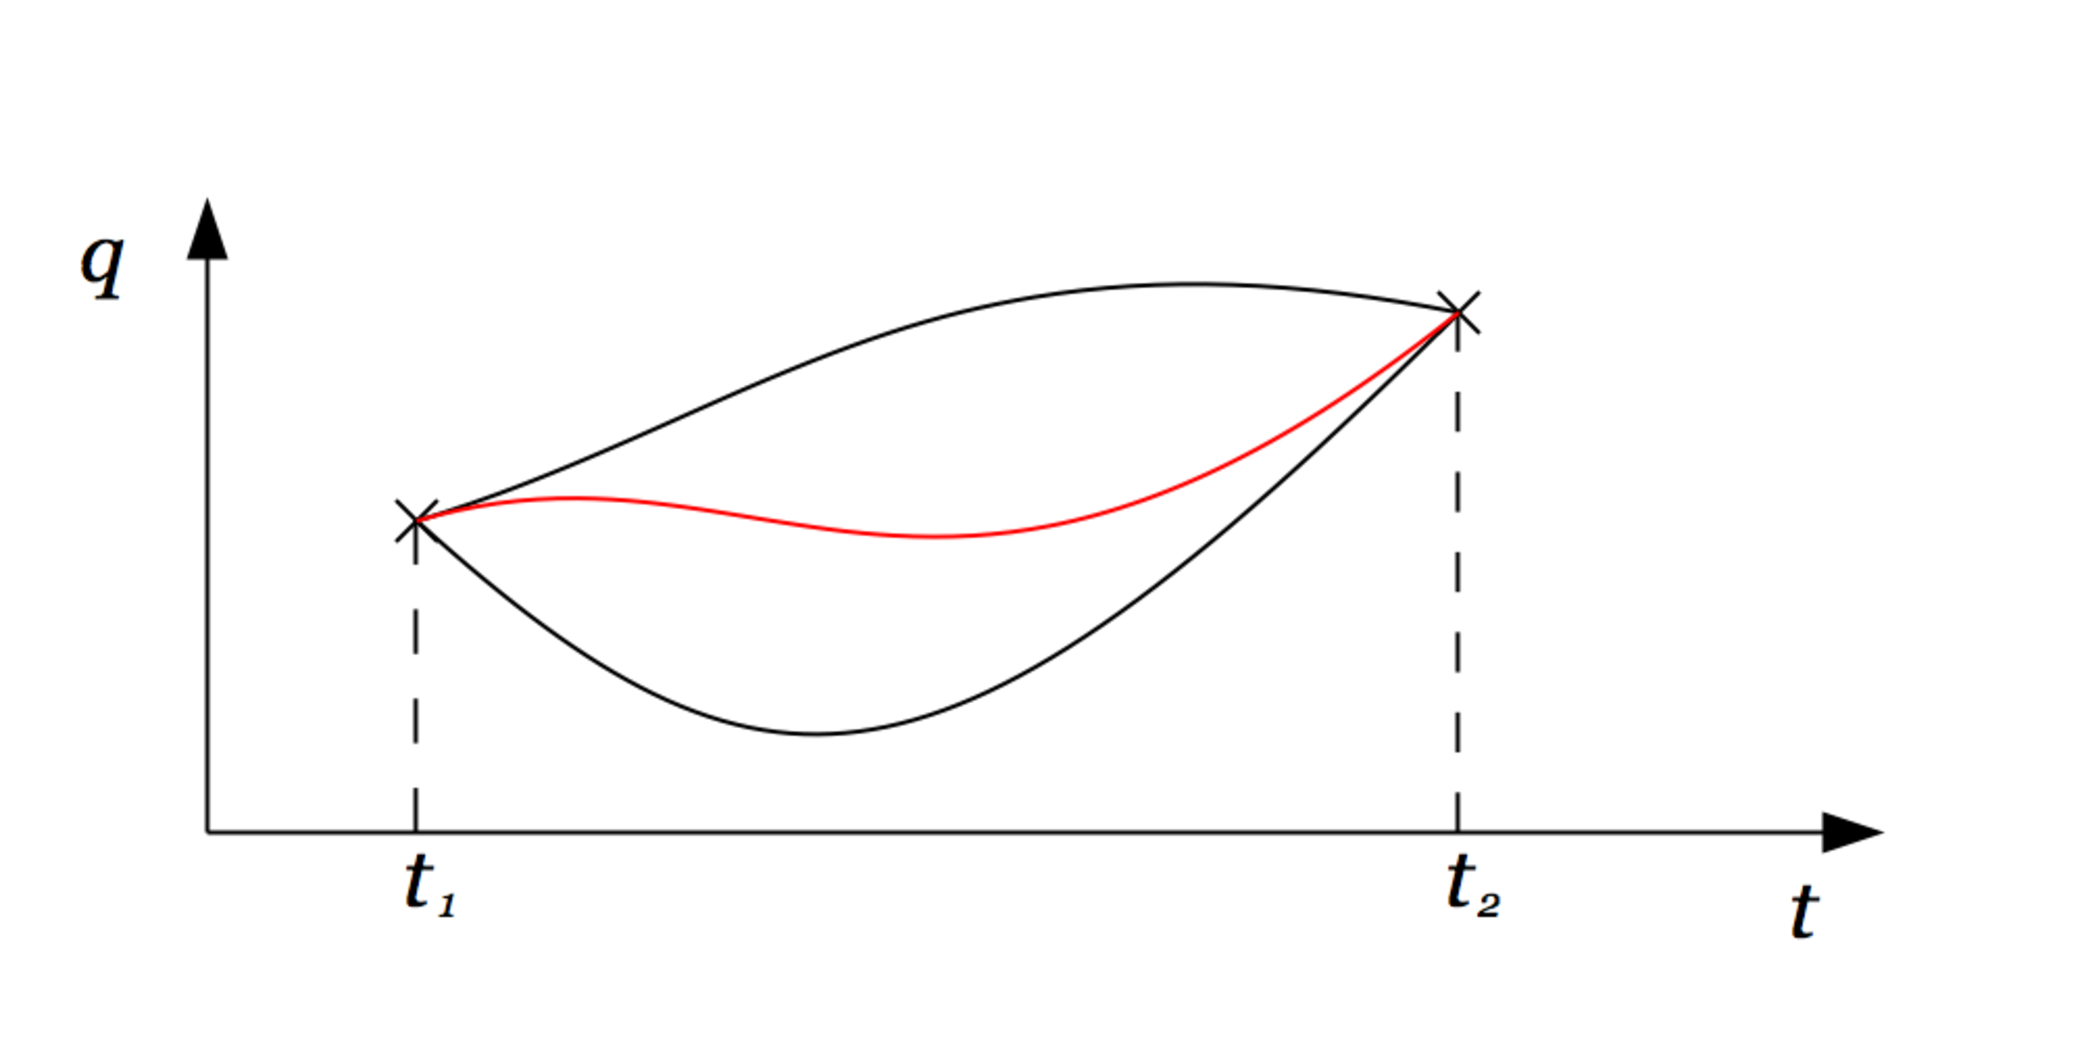
\includegraphics[width=\textwidth]{images/chapter_4/action2.pdf}
    \caption[Schematic diagram showing action]{In general several paths connect points $(x_1;t_1)$ and $(x_2;t_2)$, but the path which minimises the action is favoured.  The red path indicates the path which minimises action.}
    \label{fig:ch4_action}
  \end{center}
\end{figure}

\begin{eqnarray*}
  \textrm{If }                s & = & \int_{t_1}^{t_2}L(q,\dot{q})\mathrm{d}t \\
  \textrm{then }       \delta s & = & \int_{t_1}^{t_2}\left( \frac{\partial L}{\partial q}\delta q + \frac{\partial L}{\partial \dot{q}}\delta \dot{q}\right) \mathrm{d}t \\
  \textrm{Now }  \delta \dot{q} & = & \delta \frac{\mathrm{d}q}{\mathrm{d}t} = \frac{\mathrm{d}}{\mathrm{d}t}\left( \delta q \right) \\
  \textrm{So }         \delta s & = & \int_{t_1}^{t_2}\Bigg[ \frac{\partial L}{\partial q}\delta q + \frac{\partial L}{\partial \dot{q}}\frac{\mathrm{d}}{\mathrm{d}t}\left(\delta q \right)\Bigg] \mathrm{d}t
\end{eqnarray*}

Integration by parts gives:

\begin{eqnarray*}
  \delta s & = & \int_{t_1}^{t_2}\Bigg[ \frac{\partial L}{\partial q}\delta q + - \frac{\mathrm{d}}{\mathrm{d}t}\frac{\partial L}{\partial \dot{q}}\delta q \Bigg] \mathrm{d}t + \Bigg[ \frac{\partial L}{\partial \dot{q}}\Bigg]_{t_1}^{t_2} \\
  & = & 0 \\
  \textrm{But } \delta q(t_2) = \delta q(t_1) & = & 0 \\
  \Rightarrow \frac{\partial L}{\partial q} \delta q - \frac{\mathrm{d}}{\mathrm{d}t}\frac{\partial L}{\partial \dot{q}}\delta q & = & 0 \\
  \textrm{or } \frac{\partial L}{\partial q} - \frac{\mathrm{d}}{\mathrm{d}t}\frac{\partial L}{\partial \dot{q}} & = & \textrm{ (The Euler-Lagrange equation)}
\end{eqnarray*}

For the harmonic oscillator:

\begin{eqnarray*}
  L & = & \frac{m\dot{q}^2}{2} - \frac{m\omega^2q^2}{2} \\
  \frac{\partial L}{\partial \dot{q}} & = & m\dot{q} \\
  \frac{\partial L}{\partial q} & = & m\omega^2q \\
  \frac{\mathrm{d}}{\mathrm{d}t}\frac{\partial L}{\partial \dot{q}} = \frac{\partial L}{\partial q} \\
  \Rightarrow m\ddot{q} & = & m\omega^2q
\end{eqnarray*}

giving Newton's second law.

In quantum mechanics, dynamical variables (eg momentum) are operators, and in general do not commute.

\[
  \mathrm{Specifically}\quad \lbrack \hat{q},\hat{p} \rbrack = i
\]

where $\hat{p}$ is the generalisation:

\[
  \hat{p} = \frac{\partial L}{\partial \dot{q}}
\]

The Heisenberg equation of motion for an operator $\hat{A}$ is:

\[
  \frac{\mathrm{d}\hat{A}}{\mathrm{d}t} = i \lbrack H,\hat{A}\rbrack
\]

The Hamiltonian, defined in terms of the Lagrangian is:

\[
  H = \hat{p}\cdot\hat{\dot{q}} - L
\]

In the classical operator:

\begin{eqnarray*}
  L & = & \frac{m\hat{\dot{q}^2}}{2} - \frac{m\omega^2\hat{q}^2}{2} \\
  \frac{\partial L}{\partial \hat{\dot{q}}} & = & \hat{p} \\
  \textrm{So } H & = & \hat{p}\hat{q} - L \\
  & = & \hat{p}\hat{q} - \frac{m\hat{\dot{q}}^2}{2} + \frac{m\omega^2\hat{q}^2}{2} \\
  & = & \hat{p}\frac{\hat{p}}{m} - \frac{\hat{p}^2}{2m} + \frac{m\omega^2}{2}\hat{q}^2 \\
  \textrm{So } H & = & \frac{\hat{p}^2}{2m} + \frac{m\omega^2}{2}\hat{q}^2
\end{eqnarray*}

\subsection{The Dirac \texorpdfstring{$\delta$}{Delta} function}

The Dirac $\delta$ function may be thought of as a function of height $1/\Delta x$ and width $\Delta x$ around a value of $x = x_0$ in the limit $\Delta x \to 0$, as shown in figure \ref{fig:ch4_diracDelta}.

\begin{figure}[!htb]
  \begin{center}
    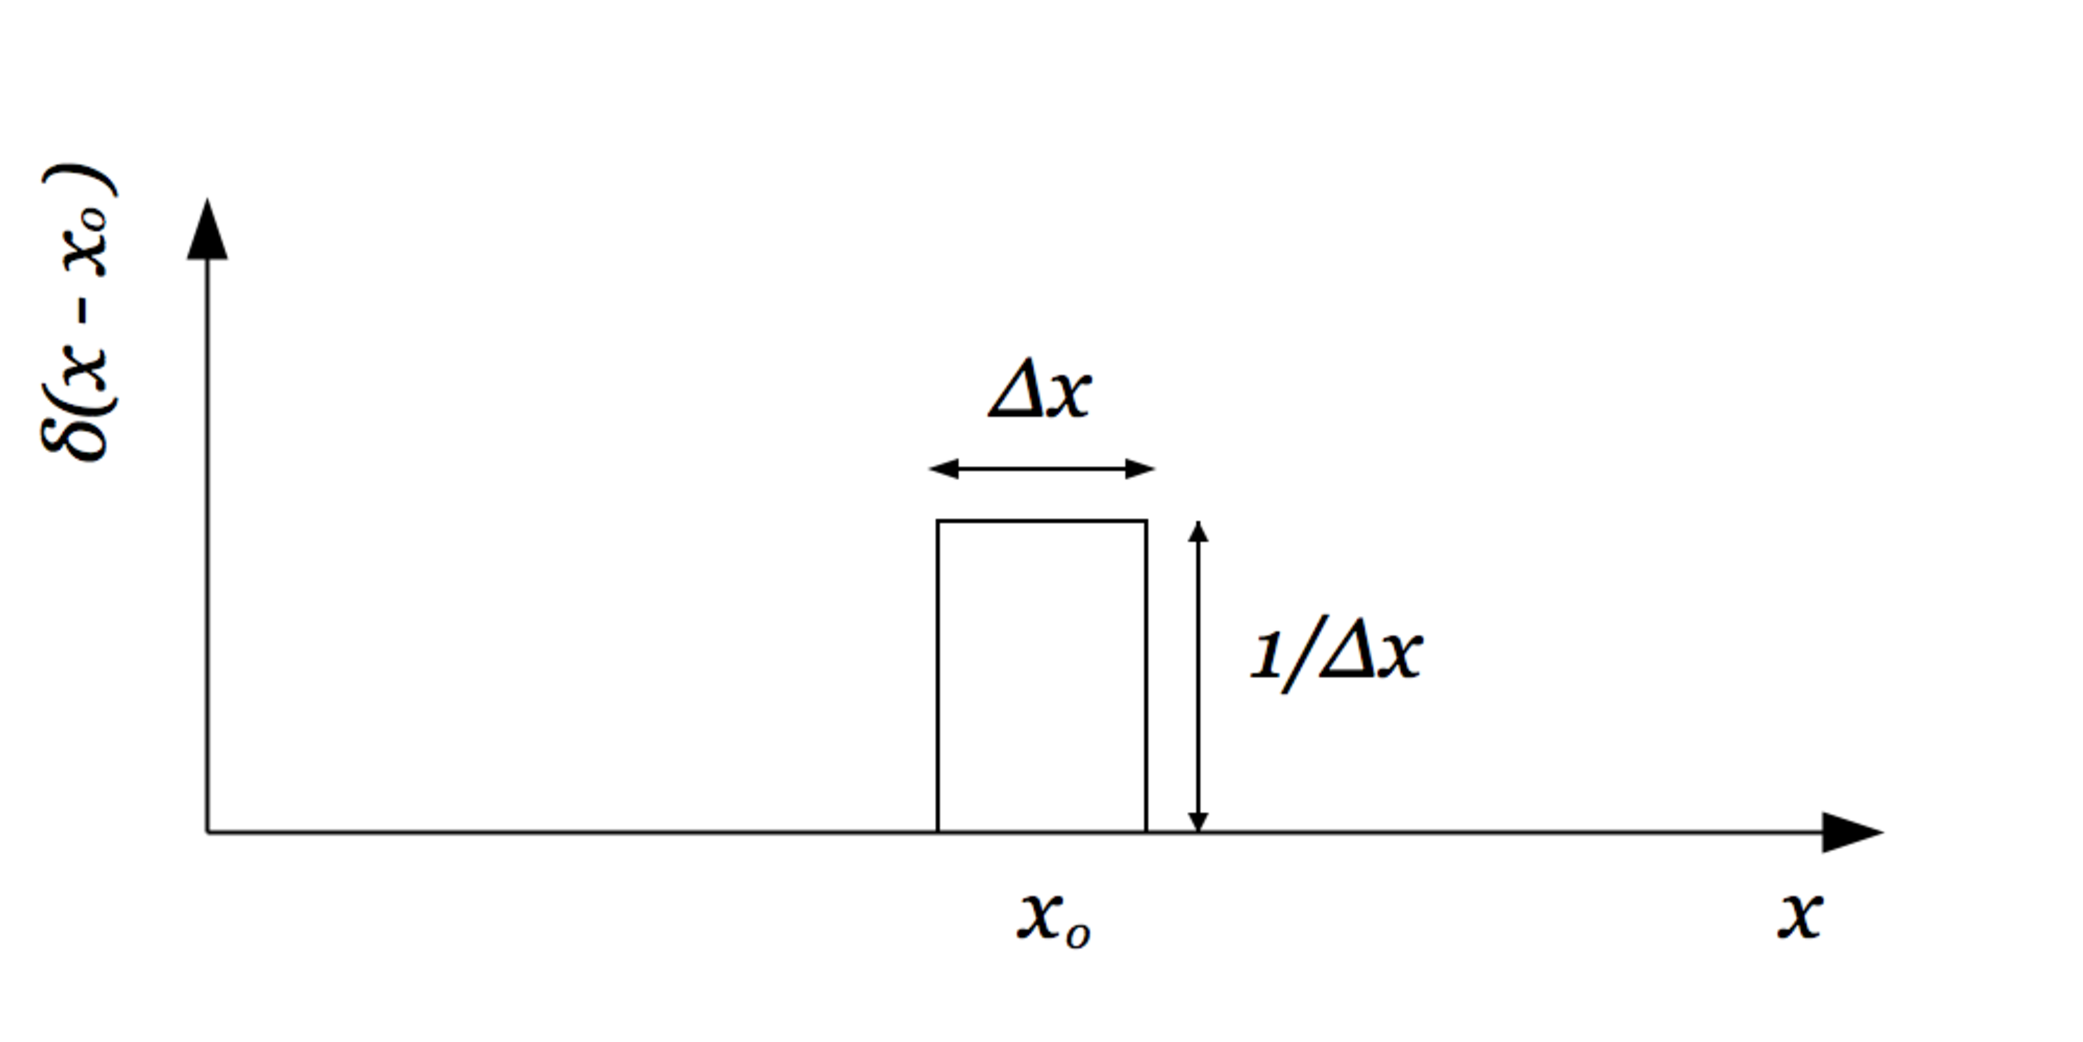
\includegraphics[width=\textwidth]{images/chapter_4/diracDelta.pdf}
    \caption[The Dirac $\delta$ function]{The Dirac $\delta$ function has width $\Delta x$ and height $1/\Delta x$ in the limit $\Delta x\to 0$.}
    \label{fig:ch4_diracDelta}
  \end{center}
\end{figure}

\[
  Area = \int \delta(x - x_0) \mathrm{d}x = 1 \\
\]

\[
  \delta(x-x_0) =
  \Bigg\{
    \begin{array}{cc}
    0 & x\neq x_0 \\
    1 & x = 0
    \end{array}{}
\]

Consider the function $f(x)$ to be split into elements $\Delta x$ wide:

\begin{eqnarray*}
  \int f(x) \mathrm{d}x & =  & \displaystyle\sum_i f(x_i) \Delta x \\
  \int f(x) \delta(x-x_0) \mathrm{d}x & = & \displaystyle\sum_i f(x_i)\delta(x_i - x_0)
\end{eqnarray*}

For the bin $x_i \neq x_0$ it is clear that $\delta(x_i - x_0) = 0$, but when $x_i = x_0$, $\delta(x_i - x_0) = 1/\Delta x$.

\begin{eqnarray*}
  \Rightarrow \int f(x)\delta(x-x_0)\mathrm{d}x & = & \lim_{x \to 0} f(x_0) \frac{1}{\Delta x}\Delta x \\
  \Rightarrow \int f(x)\delta(x-x_0)\mathrm{d}x & = & f(x_0)
\end{eqnarray*}

Some useful expressions and functions limit to the Dirac $\delta$ function:

\begin{eqnarray*}
  \delta(x) = & \displaystyle\lim_{\epsilon \to 0} \frac{1}{\epsilon} & \mathrm{ for } -\epsilon/2 < x < \epsilon/2 \\
  \delta(x) = & \displaystyle\lim_{\epsilon \to 0} \frac{1}{\pi}\frac{\epsilon}{x^2 + \epsilon^2} & \textrm{ (Breit-Wigner resonance)}
\end{eqnarray*}

Consider the Breit-Wigner resonance:

\begin{eqnarray*}
  I & = & \int_{-\infty}^{\infty} \frac{1}{\pi}\frac{\epsilon}{x^2 + \epsilon^2}\mathrm{d}x \\
  x & = & \epsilon \tan \theta \\
  \mathrm{d}x & = & \epsilon \sec^2\theta \\
  I & = & \frac{1}{\pi}\int_{\pi/2}^{\pi/2}\frac{\epsilon\epsilon\sec^2\theta}{\epsilon^2(1 + \tan^2\theta)}\mathrm{d}\theta \\
    & = & 1
\end{eqnarray*}

So it appears that the Breit-Wigner function approaches the Dirac $\delta$ function in the appropriate limit.  At $x=0$ the function has a value $1/\pi\epsilon$.  At $x=\pm\epsilon$ the function reaches the half maximum, $1/2\pi\epsilon$.  $\Gamma/2 = \epsilon$ where $\Gamma$ is the full width at half height and is more commonly used in the Breit-Wigner function.

Another form of the Dirac $\delta$ function is:

\[
  \delta(x-x_0) = \int_{-\infty}^{\infty} \frac{1}{2\pi} \e^{ik(x-x_0)} \mathrm{d}k
\]

Consider Fourier analysis of the above form.  Recall that for a well behaved function of $x$ between $-L/2$ and $L/2$ the function can be expressed as a Fourier series with wavelengths $\lambda = L$, $\frac{L}{2}$, $\frac{L}{3} \cdots$

\[
  f(x) = \displaystyle\sum^{\infty}_{x=-\infty}a_n\e^{i2\pi nx/L}
\]

To find $a_n$ integrate both sides:

\begin{eqnarray*}
  \int_{-L/2}^{L/2}\mathrm{d}xf(x)\e^{-12\pi nx/L} & = & \int_{L/2}^{L/2}a_n \mathrm{d}x \\
  \Rightarrow a_n & = & \frac{1}{L} \int_{-L/2}^{L/2}\mathrm{d}xf(x) \e^{-12\pi nx/L} \\
  \mathrm{Consider } \lim L\to \infty \\
  f(x) & = & \displaystyle\sum_{-\infty}^{\infty}a_n \e^{i2\pi nx/L}\Delta n \\
\end{eqnarray*}

where $\Delta n$ is the interval and $\Delta n = 1$

\begin{eqnarray*}
  \textrm{Define } k & = & \frac{2\pi n}{L} \\
  \mathrm{d}k & = & 2\pi \frac{\Delta n}{L} \\
  f(x) & = & \displaystyle\sum_{-\infty}^{\infty} a_n \e^{ikx} \frac{L}{2\pi} \mathrm{d}k \\
  & = & \frac{1}{2\pi} \int_{-\infty}^{\infty}\e^{ikx}g(k)\mathrm{d}k \\
  \textrm{where } g(k) & = & La_n \\
  g(k) & = & \int_{-\infty}^{\infty} f(x)\e^{-ikx} \mathrm{d}x \\
  f(x) & = & \frac{1}{2 \pi}\int_{-\infty}^{\infty} g(k)\e^{ikx}\mathrm{d}k
\end{eqnarray*}

Substituting $g(k)$ into the expression for $f(x)$:

\begin{eqnarray*}
  f(x) & = & \frac{1}{2 \pi} \int_{-\infty}^{\infty} \int_{-\infty}^{\infty}f(x')\e^{-ikx'}\e^{ikx}\mathrm{d}k\mathrm{d}x' \\
  & = & \int_{-\infty}^{\infty} f(x')\mathrm{d}x' \int_{-\infty}^{\infty} \frac{1}{2\pi} \e^{ik(x-x')}\mathrm{d}k \\
  \textrm{So } \delta(x-x') & = & \frac{1}{2 \pi} \int_{-\infty}^{\infty}\e^{ik(x-x')}\mathrm{d}k
\end{eqnarray*}

Some properties of the Dirac $\delta$ function: \nopagebreak

\begin{enumerate}
\item$\delta(ax) = \delta(x)/a$ Proof:

\begin{eqnarray*}
  \textrm{Let } ax & = & y \\
  \Rightarrow a\mathrm{d}x & = & \mathrm{d} y \\
  \textrm{So } \int_{-\infty}^{\infty}\delta(ax)\mathrm{d}x & = & \int_{-\infty}^{\infty} \delta(y)\frac{\mathrm{d}y}{a} \\
  & = & \frac{1}{a}
\end{eqnarray*}

\item $\delta(x) = \delta(-x) \Rightarrow \delta(x)$ is an even function.

\item$f(x)$ and $f'(x)$  For a function $f(x)$:

\[
  \delta(f(x)) = \displaystyle\sum_i \frac{\delta(x-a_i)}{\left(\frac{\mathrm{d}f}{\mathrm{d}x}\right)_{x=a_i}} \\
\]

where $a_i$ satisfy $f(a_i) = 0$
  
At each place where $f(x) = 0$, then:

\begin{eqnarray*}
  f(x) & = & f(a_i) + (x - a_i)\frac{\mathrm{d}f}{\mathrm{d}x} + \cdots \\
  f(a_i) & = & 0
\end{eqnarray*}

So the $\delta$ function has non-zero contributions from each of the roots $a_i$ of the form:

\begin{eqnarray*}
  \delta(f(x)) & = & \displaystyle\sum_i \delta \left( (x-a_i) \left(\frac{\mathrm{d}f}{\mathrm{d}x}\right)_{x=a_i}\right) \\
  & = & \displaystyle\sum_i \frac{\delta(x-a_i)}{\left(\frac{\mathrm{d}f}{\mathrm{d}x}\right)_{x=a_i}}
\end{eqnarray*}
\end{enumerate}

\subsection{The Heaviside step function}

The Heaviside step function is shown in figure \ref{fig:ch4_heaviside}.  It is defined as:

\begin{figure}[!htb]
  \begin{center}
    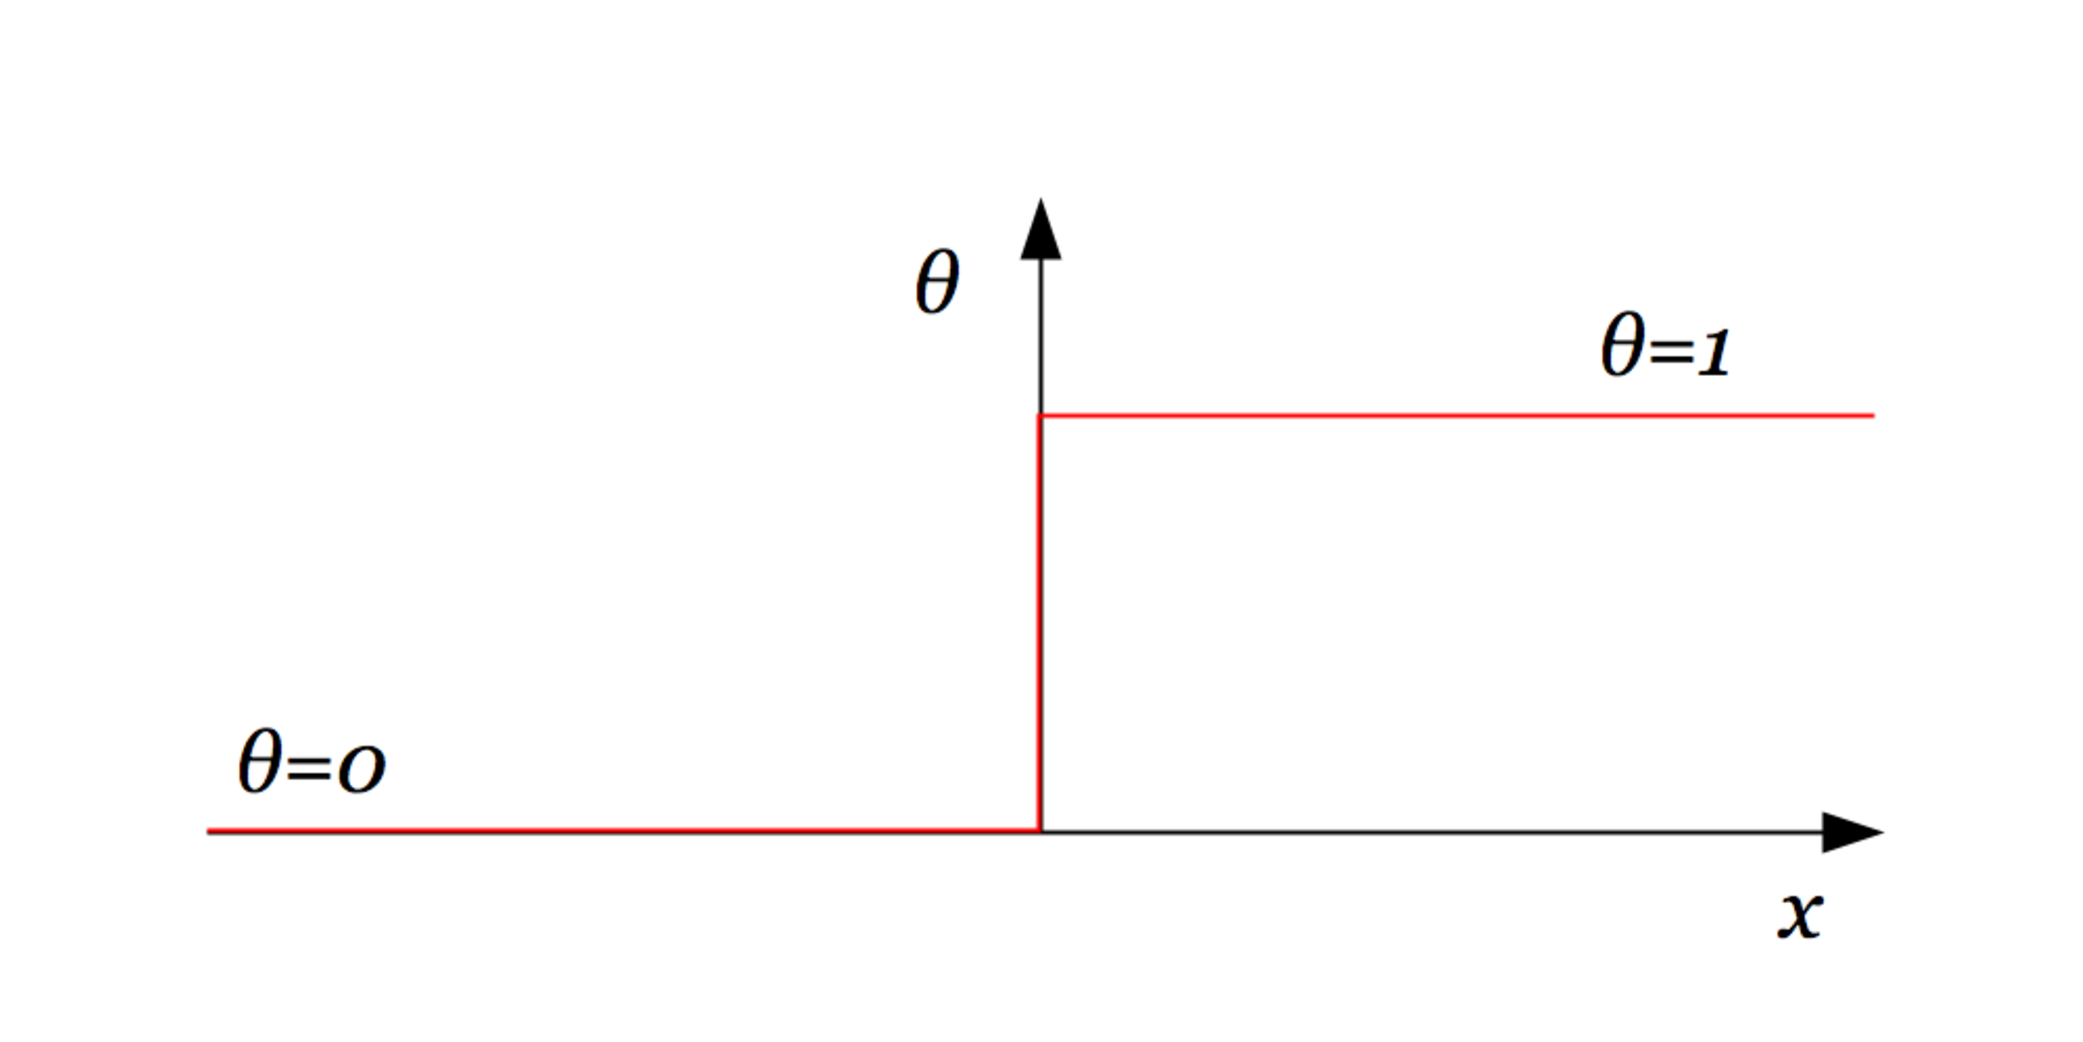
\includegraphics[width=\textwidth]{images/chapter_4/heaviside.pdf}
    \caption[The Heaviside step function]{The Heaviside step function is zero when $x<0$ and unity when $x\ge 0$.}
    \label{fig:ch4_heaviside}
  \end{center}
\end{figure}

\begin{eqnarray*}
  \theta(\tau) & = &
  \left\{
    \begin{array}{cc}
    1 & \tau>0 \\
    0 & \tau<0
    \end{array}
  \right.
  \\
  \frac{\mathrm{d}\theta}{\mathrm{d}\tau} & = & \delta (\tau) \\
  & = & \frac{1}{2\pi} \int_{-\infty}^{\infty}\e^{-i\omega\tau}\mathrm{d}\omega \\
  \Rightarrow \theta & = & \frac{1}{2\pi}\int_{-\infty}^{\infty}\int_{-\infty}{\infty}\e^{-i\omega\tau}\mathrm{d}\omega \mathrm{d}\tau \\
  & = & \frac{1}{2\pi} \int_{-\infty}^{\infty} \frac{\e^{-i\omega\tau}}{-i\omega}\mathrm{d}\omega \\
  \theta & = & \frac{-1}{2\pi i}\int_{-\infty}^{\infty} \frac{\e^{-\omega\tau}\mathrm{d}\omega}{\omega + i\epsilon} \\
\end{eqnarray*}

Using Cauchy's theorem gives:

\begin{eqnarray*}
  \oint_C \frac{f(z)\mathrm{d}z}{z-a} & = & 2\pi i f(a) \\
  \textrm{So } \theta & = & \frac{-1}{2\pi i} \left(-2ni\e^{(-i\tau)(-i\epsilon)}\right) \\
  & = & \e^{-\epsilon\tau} \\
  \textrm{For } \epsilon \to 0, \theta & = & 1
\end{eqnarray*}
